%%%%%%%%%%%%%%%%%%%%%%%%%%%%%%%%%%%%%%%%%%%%%%%%%%%%%%%%%%%%%%%%%%%%%%
% Lớp 10 | Hàm số bậc hai và đồ thị | Hàm số và đồ thị
% Dạng 0D3?1-4: Đồ thị của hàm số
% Số câu: 11  (sinh tự động bởi tach_cau.py; từ nay thầy sửa trực tiếp file này)
%%%%%%%%%%%%%%%%%%%%%%%%%%%%%%%%%%%%%%%%%%%%%%%%%%%%%%%%%%%%%%%%%%%%%%

%%%%%%%%%%%%%%%% TRẮC NGHIỆM 4 PHƯƠNG ÁN %%%%%%%%%%%%%%%%

% nguồn: MaHoaNH_TracNghiem_Lop10
\begin{ex}%[0D3N1-4]%[ma:5dfd96e7]
	Tọa độ giao điểm của hai đường thẳng $y=\dfrac{1-3x}{4}$  và $y=-\left(\dfrac{x}{3}+1\right)$ là
	\choice 
		{$(0;-1)$} 
		 {$(2;-3)$}
		{$(0;\dfrac{1}{4})$} 
		{\True $(3;-2)$} 
	 \loigiai{
		Phương trình hoành độ giao điểm của  hai đường thẳng $$\dfrac{1-3x}{4}=-\left(\dfrac{x}{3}+1\right)\Leftrightarrow x=3 \Rightarrow y=-2.$$
	Vậy tọa độ giao điểm của  hai đường thẳng là $(3;-2)$.}
\end{ex}

% nguồn: MaHoaNH_TracNghiem_Lop10
\begin{ex}%[0D3N1-4]%[ma:e5fee7be]
	Cho parabol $(P)\colon y=3x^{2}-2x+1$. Điểm nào sau đây  thuộc $(P)$?
	\choice 
		{\True $I(1;2)$} 
		 {$A(0;-1)$}
		{$B\left(  -\dfrac{1}{3};\dfrac{2}{3}\right) $}
		{$C\left(  \dfrac{1}{3};-\dfrac{2}{3}\right) $}
	\loigiai{Thay tọa độ điểm $I(1;2)$ vào phương trình  parabol $(P)$, ta có
		 $2 = 3(1)^2 - 2(1) + 1 \Leftrightarrow 2 = 2$.\\
	Vậy điểm $I(1;2)$ thuộc  parabol $(P)$.}
\end{ex}

% nguồn: MaHoaNH_TracNghiem_Lop10
\begin{ex}%[0D3N1-4]%[ma:94da43cb]
	 Tọa độ giao điểm của hai đường thẳng $y=x+2$ và $y=-\dfrac{3}{4}x+3$ là
	\choice 
		{$\left(-\dfrac{4}{7};-\dfrac{18}{7}\right)$} 
		 {$\left(\dfrac{4}{7};-\dfrac{18}{7}\right)$}
		 {$\left(-\dfrac{4}{7};\dfrac{18}{7}\right)$}
		 {\True $\left(\dfrac{4}{7};\dfrac{18}{7}\right)$}
	\loigiai{ 
		Phương trình hoành độ giao điểm của hai đường thẳng là $x+2=-\dfrac{3}{4}x+3\Leftrightarrow x=\dfrac{4}{7}$.\\ 
		 Suy ra $y=\dfrac{4}{7}+2=\dfrac{18}{7}$.\\
	Vậy tọa độ giao điểm của hai đường thẳng là  $\left(\dfrac{4}{7};\dfrac{18}{7}\right)$.}
\end{ex}

% nguồn: MaHoaNH_TracNghiem_Lop10
\begin{ex}%[0D3H1-4]%[ma:b07d4333]
	Đường thẳng $y=2-x$ tạo với hai trục tọa độ một tam  giác có diện tích bằng
	 \choice
		 {$1$}
		{$2{,}5$} 
		{$4$} 
		{\True  $2$}
	 \loigiai{
		Giao với trục $Ox$ tại  điểm $A(2;0)$.\\
		Giao với trục $Oy$ tại điểm $B(0;2)$.\\ 
		Khi đó độ dài các cạnh $OA=2$, $OB=2$.\\ 
	Ta có tam giác $OAB$  vuông tại $O$ nên $S_{OAB}=\dfrac{1}{2}OA.OB=2$.}
\end{ex}


%%%%%%%%%%%%%%%% ĐÚNG/SAI %%%%%%%%%%%%%%%%

% nguồn: MaHoaNH_DungSai_Lop10
\begin{ex}%[0D3H1-4]%[ma:b5e8e007]
	\immini{Cho hàm số $y=f(x)$ có đồ thị như hình vẽ bên. Mỗi kết quả dưới đây đúng hay sai?}{ 
	\begin{tikzpicture}[scale=1,font=\footnotesize,line join=round,line cap=round,>=stealth]
			\draw  [->] (-3,0)--(3,0) node[below]{$x$};
			\draw  [->] (0,-2)--(0,2) node[left]{$y$};
			 \draw[fill=black] (0,0) circle (1pt) node[below left]{$O$};
			\clip (-3,-2) rectangle  (3,2);
			\draw[name path=c1,smooth,samples=300,domain=-3:0] plot (\x,{-1}); 
			\draw[name  path=c2,smooth,samples=300,domain=1:3] plot (\x,{1});
			 \draw (0,-1)--(1,1);
			\foreach \i  in {-2,-1,1,2} \draw [fill=black] (\i,0) circle (1pt) node[below]{$\i$};
			\foreach \j in {1}  \draw [fill=black] (0,\j) circle (1pt) node[left]{$\j$};
			\draw[fill=black] (0,-1) circle  (1pt) node[right]{$-1$};
			\draw[fill=black] (1,1) circle (1pt); 
		\end{tikzpicture}
	} 
	 \choiceTF
		 {$f(1)=0$}
		{\True $f(-2)<f(2)$} 
		{\True Điểm $\left(-2024;-1\right)$ thuộc đồ thị hàm số} 
		 {\True $-1\le f(x)$, $\forall x\in\mathscr{D}$}
	\loigiai{ 
		\begin{itemchoice}
			 \itemch $f(1)=1$.
			\itemch  Do $f(-2)=-1<f(2)=1$.
			\itemch Từ đồ thị của hàm số suy ra điểm $\left(-2024;-1\right)$ thuộc đồ  thị hàm số.
			\itemch Từ đồ thị ta  có $f(x)\ge -1$.
		\end{itemchoice}
	 }
\end{ex}

% nguồn: MaHoaNH_DungSai_Lop10
\begin{ex}%[0D3H1-4]%[ma:4648d2b3]
	\immini{Cho hàm số $y=f(x)$ có đồ thị như hình vẽ bên. Mỗi kết quả  dưới đây đúng hay sai?}{
	\begin{tikzpicture}[scale=0.4,font=\footnotesize,line join=round,line cap=round,>=stealth]
			\draw [->] (-3,0)--(10,0)  node[below]{$x$};
			 \draw [->] (0,-3)--(0,9) node[right]{$y$};
			 \draw[fill=black] (0,0) circle (1pt) node[below left]{$O$};
			 \draw[opacity=0.1] (-3,-3) grid (10,9);
			\clip  (-5,-3) rectangle (11,8);
			\draw[name path=c1,smooth,samples=300,domain=-1:5]  plot (\x,{0.5*(\x)^2-1.5*(\x)+3});
			\draw  (5,-2)--(9,6);
			\foreach \i in {-2,2,4,6,8} \draw  [fill=black] (\i,0) circle (1pt) node[below]{$\i$};
			\foreach \j in {-2,4,6} \draw [fill=black] (0,\j) circle  (1pt) node[left]{$\j$};
			\draw  [fill=black] (0,2) circle (1pt) node[right]{$2$};
			 \draw [fill=black](-1,1) circle (1pt);
			\draw [fill=black](9,6) circle  (1pt);
			\draw [fill=black](0,3)  circle (1pt);
		\end{tikzpicture}
	} 
	 \choiceTF
		{\True $f(x)=0\Leftrightarrow x= 6$} 
		{$f(5)=-2$} 
		{Tập xác định  $\mathscr{D}=\left[-1;5\right)$}
		{\True $-2\le f(x)\le  8$, $\forall x\in\mathscr{D}$}
	\loigiai{ 
		\begin{itemchoice}
			\itemch Đồ  thị hàm số $y=f(x)$ cắt trục hoành tại điểm có hoành độ $x=6$.
			\itemch Từ đồ thị hàm số $y=f(x)$ thì $f(5)$ không tồn tại. 
			\itemch Hàm số xác định với $x\in\left(5;9\right]$. 
			 \itemch Từ đồ thị ta có $-2\le f(x)\le 8$.
		\end{itemchoice}
	} 
\end{ex}

% nguồn: MaHoaNH_DungSai_Lop10
\begin{ex}%[0D3H1-4]%[ma:c2b83053]
	\immini{Cho hàm số  $y=f(x)$ có đồ thị như hình vẽ bên. Mỗi kết quả dưới đây đúng hay sai?}{
	\begin{tikzpicture}[scale=0.4,font=\footnotesize,line join=round,line cap=round,>=stealth]
			\draw [->] (-3,0)--(10,0) node[below]{$x$}; 
			\draw [->] (0,-3)--(0,7)  node[right]{$y$};
			\draw[fill=black] (0,0) circle (1pt)  node[below left]{$O$};
			\draw[opacity=0.1] (-3,-3) grid (10,7); 
			\clip  (-5,-3) rectangle (11,8);
			 \draw[name path=c1,smooth,samples=300,domain=-1:5] plot (\x,{-0.5*(\x)^2+1.5*(\x)+3});
			\draw  (5,-2)--(9,6);
			\foreach \i in {-2,2,4,6,8} \draw  [fill=black] (\i,0) circle (1pt) node[below]{$\i$};
			\foreach \j in {-2,4,6} \draw [fill=black] (0,\j) circle (1pt) node[left]{$\j$}; 
			\draw [fill=black] (0,2) circle (1pt)  node[right]{$2$};
			\draw [fill=black](-1,1)  circle (1pt);
			\draw [fill=black](9,6) circle (1pt); 
			\draw [fill=black](5,-2) circle (1pt); 
			\draw [fill=black](0,3)  circle (1pt);
		\end{tikzpicture}
	 }
	 \choiceTF
		{$f(x)=0\Leftrightarrow x=  6$}
		{\True $f(0)=3$} 
		{\True Tập xác  định $\mathscr{D}=\left[-1;9\right]$}
		{  $f(x)\ge 2$, $\forall x\in\mathscr{D}$}
	 \loigiai{
		\begin{itemchoice}
			\itemch Đồ thị hàm số $y=f(x)$ cắt trục hoành  tại hai điểm phân biêt.
			 \itemch $f(0)=3$.
			\itemch Từ đồ thị suy  ra $\mathscr{D}=\left[-1;9\right]$
			\itemch  $f(x)\ge -2$.
		\end{itemchoice}
	 }
\end{ex}

% nguồn: MaHoaNH_DungSai_Lop10
\begin{ex}%[0D3H1-4]%[ma:e395be2c]
	\immini{Cho hàm số $y=f(x)$ có đồ thị như hình vẽ bên.  Mỗi kết quả dưới đây đúng hay sai?}{
	\begin{tikzpicture}[font=\footnotesize,line join=round,line cap=round,>=stealth,scale=1]
			\draw[->] (-2,0) -- (3,0)  node[below] {$x$};
			\draw[->] (0,-3) -- (0,1.5) node[left] {$y$}; 
			\begin{scope}
				 \clip (-2.5,-2.5) rectangle (3,2);
				\draw[samples=200,domain=-2: 5,smooth,variable=\x] plot  (\x,{-(\x)^2+1*(\x)})
					(-1.2,-2) node[above]  {$(P)$};
			\end{scope}
			\foreach  \x/\y in{0/0,1/0,2/0,0/1}{
				\fill (\x,\y) circle (1.5pt); 
			} 
			\path 
				 node at (0,0)[above left]{$O$}
				node at (1,0)[below left]{$1$} 
				node at (2,0)[below]{$2$} 
				node at  (0,1)[left]{$1$};
		\end{tikzpicture}
	} 
	\choiceTF 
		{\True  $f(x)=0\Leftrightarrow \hoac{&x=0\\&x=1}$}
		 {$f(0)=1$}
		{\True  Hàm số đồng biến trên $\left(-\infty;0\right)$}
		 {$1\le f(x)$, $\forall x\in\mathscr{D}$}
	\loigiai{ 
		\begin{itemchoice}
			 \itemch Đồ thị hàm số $y=f(x)$ cắt trục hoành tại hai điểm có hoành độ $x=0$ và $x=1$.
			\itemch Từ đồ  thị hàm số $y=f(x)$ thì $f(0)=0$.
			\itemch Từ đồ thị của hàm số suy ra hàm  số đồng biến trên $\left(-\infty;0\right)$.
			\itemch Từ đồ thị  ta có $f(x)<1$.
		\end{itemchoice}
	} 
\end{ex}

% nguồn: MaHoaNH_DungSai_Lop10
\begin{ex}%[0D3H1-4]%[ma:254341cb]
	\immini{Cho hàm số $y=f(x)$  có đồ thị như hình vẽ bên. Mỗi kết quả dưới đây đúng hay sai?}{
	\begin{tikzpicture}[font=\footnotesize,line join=round,line cap=round,>=stealth,scale=1]
			\draw[->]  (-2,0) -- (2,0) node[below] {$x$};
			\draw[->] (0,-2.2) --  (0,2.5) node[left] {$y$};
			\begin{scope}
				\clip (-2.5,-2.5)  rectangle (3,2);
				\draw[samples=200,domain=-2: 5,smooth,variable=\x] plot (\x,{(\x)^4-2*(\x)^2-1}); 
			\end{scope}
			 \draw[dashed] (1,0)--(1,-2)--(-1,-2)--(-1,0);
			\foreach \x/\y  in{0/0,1/0,-1/0,0/-1,0/-2,1/-2,-1/-2}{
				 \fill (\x,\y) circle (1.5pt);
			 }
			\path 
				node  at (0,0)[above left]{$O$}
				node  at (1,0)[below left]{$1$}
				node  at (-1,0)[above]{$-1$}
				node at (0,-1)[above left]{$-1$} 
				 node at (0,-2)[above left]{$-2$};
		\end{tikzpicture}
	 }
	 \choiceTF
		{Phương trình $f(x)=0$ có  $4$ nghiệm phân biệt}
		{\True $f(2)=f(-2)$} 
		{\True Hàm số nghịch  biến trên $\left(0;1\right)$}
		{\True $-2\le f(x)$, $\forall  x\in\mathscr{D}$}
	\loigiai{ 
		\begin{itemchoice}
			\itemch Đồ thị  hàm số $y=f(x)$ cắt trục hoành tại hai điểm có hoành độ $x=0$ và $x=1$.
			\itemch Từ đồ thị hàm số  $y=f(x)$ thì $f(0)=0$.
			\itemch Từ đồ thị của hàm số suy ra hàm số  đồng biến trên $\left(-\infty;0\right)$.
			\itemch Từ đồ thị ta  có $f(x)<1$.
		\end{itemchoice}
	 }
\end{ex}

% nguồn: MaHoaNH_DungSai_Lop10
\begin{ex}%[0D3H1-4]%[ma:e4c54c1d]
	Cho hàm số ${y=f(x)}$ có  đồ thị là đường gấp khúc như hình bên dưới.
	\begin{center}
		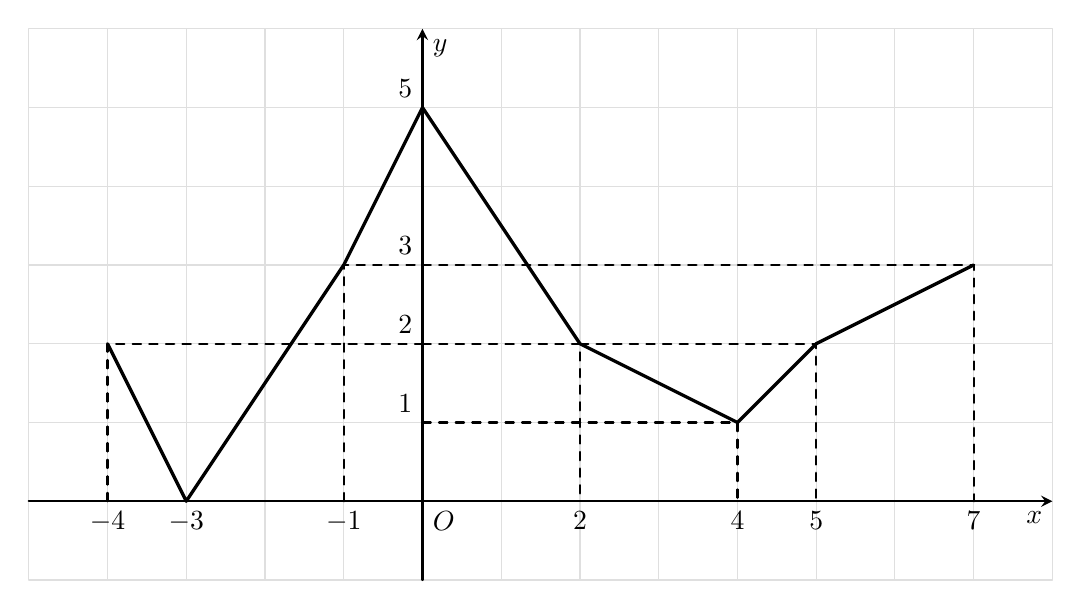
\begin{tikzpicture}[line join=round,line cap=round,thick]
				 \draw[gray!50,thin,opacity=.5]
					(-5,-1)  grid (8,6);
				\draw [-stealth,thick](-5,0) -- (8,0)  node[below left]{$x$};
				\draw  [-stealth,thick](0,-1) -- (0,6) node[below right]{$y$};
				\draw[very thick]  (-4,2)--(-3,0)--(-1,3)--(0,5)--(2,2)--(4,1)--(5,2)--(7,3);
				\draw[dashed] (-4,0) node[below]{$-4$}|-(0,2) node[above left]{$2$} 
					(-1,0) node[below]{$-1$}|-(0,3) node[above  left]{$3$}
					(0,2)-|(2,0) node[below]{$2$} 
					 (0,1) node[above left]{$1$}-|(4,0) node[below]{$4$}
					(2,2)--(5,2)--(5,0) node[below]{$5$} 
					(0,3)-|(7,0) node[below]{$7$} 
					(0,0) node[below right]{$O$} 
					 (-3,0) node[below]{$-3$}
					(0,5) node[above  left]{$5$};
			\end{tikzpicture}
	\end{center}
	Khi đó 
	\choiceTF 
		{Tập giá trị hàm số  $T=[-4;7]$}
		{\True Ta thấy điểm $(-4;2)$, $(4;1)$ thuộc đồ thị hàm số, điểm $(2;3)$ không thuộc đồ thị hàm  số}
		{\True Ta  có $f(-1)=3$, $f(5)=2$}
		{\True Hàm số đã  cho đồng biến trên các khoảng $(-3;0)$, $(4;7)$; hàm số nghịch biến trên các khoảng $(-4;-3)$, $(0;4)$}
	\loigiai{ 
		\begin{itemchoice}
			\itemch Tập xác định hàm  số $\mathscr{D}=[-4;7]$. Tập giá trị hàm số $T=[0;5]$.
			\itemch Ta thấy điểm $(-4;2)$, $(4;1)$  thuộc đồ thị hàm số, điểm $(2;3)$ không thuộc đồ thị hàm số.
			\itemch Ta có  $f(-1)=3$, $f(5)=2$.
			\itemch Hàm số đã cho đồng biến trên các khoảng $(-3;0)$, $(4;7)$; hàm số nghịch biến trên  các khoảng $(-4;-3)$, $(0;4)$.
		\end{itemchoice}
	} 
\end{ex}

% nguồn: MaHoaNH_DungSai_Lop10
\begin{ex}%[0D3H1-4]%[ma:5d8fcdb6]
	\immini{Cho đồ thị các hàm số $y=-3x+2$; $y=3x^2$.  Khi đó
	\choiceTF 
		 {Đồ thị hàm số $y=-3x+2$ là một đường cong}
		{\True Đồ thị hàm số $y=-3x+2$ cắt đồ thị hàm số $y=3x^2$ tại hai điểm} 
		{\True Đồ thị của hàm số $y=-3x+2$ nghịch biến trên  $\mathbb{R}$}
		{Đồ thị  hàm số $y=3x^2$ nghịch biến trên khoảng $(0;+\infty)$}}
		{		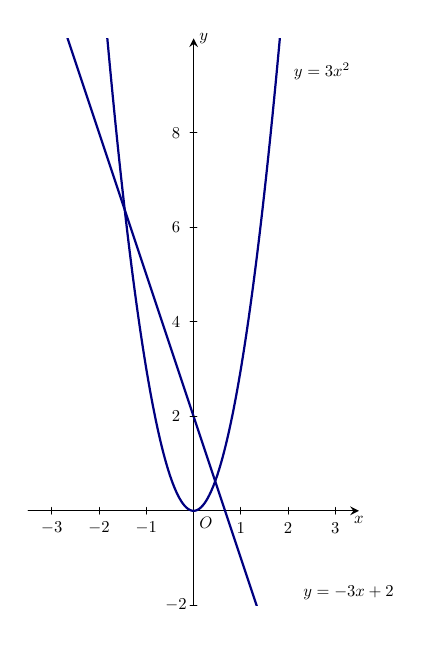
\begin{tikzpicture}[join = round,cap = round,>=stealth,transform shape,scale = 0.6]
		 \def\xmin{-3.5} \def\xmax{3.5}
		 \def\ymin{-2} \def\ymax{10}
		 \def\f (#1){3*(#1)^2}
		\def\g (#1){-3*(#1)+2} 
		\draw[->]  (\xmin,0)--(0,0) node[below right]{$O$}--(\xmax,0) node[below]{$x$};
		\draw[->] (0,\ymin)--(0,\ymax) node[right]{$y$}; 
		\begin{scope}
			\clip (\xmin,\ymin)  rectangle (\xmax,\ymax);
			\draw[smooth,thick,blue!50!black] plot[domain =  \xmin:\xmax,samples = 200,variable=\x]({\x},{\f (\x)}) node[below left] {$y=3x^2$};
			\draw[smooth,thick,blue!50!black] plot[domain = \xmin:\xmax,samples  = 200,variable=\x]({\x},{\g (\x)}) node{$y=-3x+2$};
		\end{scope}
		\foreach \x in  {}{
			\pgfmathsetmacro\fx{\f (\x)} 
			 \draw[dashed,thin] (\x,0) |- (0,{\fx});
		 }
		\foreach \x in {}{ 
			 \pgfmathsetmacro\gx{\g (\x)}
			\draw[dashed,thin] (\x,0)  |- (0,{\gx});
		 }
		\draw (\xmax-1.5,\ymax-1) node [above  right]{$y=3x^2$};
		\draw (\xmax-1.3,\ymin)  node [above right]{$y=-3x+2$};
		 \foreach \x/\g in {-3/-90,-2/-90,-1/-90,1/-90,2/-90,3/-90}
		\draw[thin] (\x,2pt)--(\x,-2pt) + (\g:3mm) node {$\x$}; 
		\foreach  \y/\g in {-2/180,2/180,4/180,6/180,8/180}
		\draw[thin]  (2pt,\y)--(-2pt,\y) + (\g:3mm) node {$\y$};
	\end{tikzpicture}}
	\loigiai{ 
		\begin{itemchoice}
			\itemch \textbf{Sai}. Đồ thị hàm số $y=-3x+2$  là một đường thẳng.
			\itemch \textbf{Đúng}. Đồ thị hàm  số $y=-3x+2$ cắt đồ thị hàm số $y=3x^2$ tại hai điểm.
			\itemch \textbf{Đúng}.Đồ thị của  hàm số $y=-3x+2$ nghịch biến trên $\mathbb{R}$.
			 \itemch \textbf{Sai}. Đồ thị hàm số $y=3x^2$ không nghịch biến trên khoảng $(0;+\infty)$.
		\end{itemchoice}
	 }
\end{ex}
